
%2%%2%%2%%2%%2%%2%%2%%2%%2%%2%%2%%2%%2%%2%%2%%2%%2%%2%%2
%               Fundamentação teórica                  %
%2%%2%%2%%2%%2%%2%%2%%2%%2%%2%%2%%2%%2%%2%%2%%2%%2%%2%%2

\chapter{Fundamentação teórica}

\label{chap:theorical}

Este capítulo tem o intuito de discutir os principais conceitos abordados nesta dissertação. A partir dele, construímos a base teórica para esta pesquisa. Falamos acerca das habilidades no contexto profissional, focando no que são soft skills e por que são importantes para qualificação profissional. Também descrevemos o Modelo dos Cinco Fatores (Five Factor Model – FFM), que trata-se de uma teoria psicológica a respeito da personalidade.

\section{Habilidades profissionais}
\label{sec:sskills}

Todo profissional possui um conjunto de habilidades que são necessárias para o desempenho de suas funções. Elas podem ser adquiridas através de estudo, treinamento ou com a prática. Nesse contexto, cada área de atuação requer habilidades específicas que tornam-se essenciais para execução das tarefas atribuídas a cada profissão.

Podemos definir essas habilidades em duas categorias: hard skills e soft skills. O termo hard skills refere-se a habilidades técnicas e conhecimentos específicos de cada profissão. Esse tipo de habilidade é aprendida e desenvolvida por meio de cursos, através da leitura de livros, estudos, observação e treinamento. Inclui, por exemplo, ser capaz de interpretar um monitor cardíaco para um médico, ou programar um site para um desenvolvedor de software.

Por outro lado, as soft skills são habilidades não-técnicas que estão relacionadas com traços de personalidade e inteligência emocional. Normalmente, são difíceis de serem ensinadas, pois se desenvolvem com a prática, através de experiências de vida que influenciam as atitudes. São exemplos de soft skills, habilidades de comunicação, liderança, autocontrole, confiança, persistência, etc. A seguir vamos detalhar esse conceito.

\subsection{Soft skills}
\label{subsec:ss}

No contexto de Tecnologia da Informação (TI), o desempenho eficaz no trabalho não envolve apenas possuir habilidades técnicas, mas também habilidades não-técnicas ou soft skills. Na literatura, outras descrições comuns para soft skills incluem os termos ``habilidades pessoais'' ou ``habilidades gerais'' \cite{joseph:99}.

Norman Cousins, um professor da University of California, Los Angeles (UCLA), pioneiro no campo de Psiconeuroimunologia (campo da ciência que se preocupa com o relacionamento entre o cérebro e o sistema imunológico) \cite{crosbie:05}, citou:

%\begin{flushright}
%\begin{minipage}{0.75\textwidth} % 75% de 160; margem para citações longas
%\begin{quotation}
\begin{quote}
``As palavras `hard' e `soft' são geralmente utilizadas por estudantes de medicina para descrever o contraste entre a natureza dos cursos. Cursos como bioquímica, física, farmacologia, anatomia e patologia são ungidos com a bênção de `hard' (difícil), enquanto temas como ética médica, filosofia, história, e relacionamento médico-paciente tendem a trabalhar sob o rótulo muito menos auspicioso `soft' (fácil) 
... [Mas] uma ou duas décadas depois da formatura, tende a haver uma inversão. O que supostamente era difícil acaba por ser fácil, e vice-versa.
A base do conhecimento de medicina está em constante mudança... Mas os temas fáceis - especialmente aqueles que têm a ver com valores intangíveis - acabam por ser de valor duradouro.''
\end{quote}
%\end{quotation}
%\end{minipage}
%\end{flushright}

A observação de Cousins ressalta que devido a constantes mudanças e novas descobertas na área de medicina é preciso evoluir, aprender e reaprender as habilidades técnicas. Isso também é verdade em outros campos e profissões. Considerando a área de TI, percebemos o surgimento e avanço de novas tecnologias em linguagens de programação, bancos de dados, desenvolvimento web, etc., o que leva o profissional dessa área à necessidade de atualizar e renovar hard skills.

Por outro lado, quando trata-se de habilidades não-técnicas, percebemos que estas possuem um valor durador. Independente dos avanços da tecnologia e da ciência ou do passar dos anos, as características definidas pelas soft skills continuarão sendo importantes da mesma maneira.

As soft skills estão relacionadas com a inteligência emocional de um indivíduo \cite{hjyunus:12}. Inteligência emocional surgiu do conceito de inteligência social. Edward Lee Thorndike foi o psicólogo americano que, em 1920, definiu inteligência social como a habilidade de compreender e administrar adequadamente os relacionamentos humanos, os quais implicam na capacidade de conviver e comunicar-se com seus semelhantes e de aproximar-se de outras pessoas \cite{thornlike:20}.

Salovey e Mayer utilizam o termo inteligência emocional para descrever a capacidade das pessoas ao lidar com as emoções, conceituando como o ``subconjunto da inteligência social que envolve a capacidade de monitorar emoções, sentimentos próprios e de outros, para discriminar entre eles e usar esta informação para orientar o pensamento e as ações'' \cite{salovey:90}.

Em outras palavras, é reconhecer os próprios sentimentos e os dos outros, e ter a capacidade de lidar com eles. Por exemplo, é ser capaz de motivar-se, controlar impulsos, regular o próprio estado de espírito e impedir que a aflição invada a capacidade de pensar. ``No mundo atual, não basta ser inteligente, esperto e preparado para competir. É preciso ter calma e empatia e persistir diante das frustrações para conseguir viver bem no amor, ser feliz com a família e vencer no mercado de trabalho'', argumenta Goleman em seu livro sobre inteligência emocional \cite{goleman:07}.

Joseph et al. \cite{joseph:99, joseph:10} definem o significado das soft skills como um conjunto de estratégias para gerenciamento de diversos aspectos no contexto do trabalho. Eles propõem um framework conceitual que caracteriza as soft skills em termos de quatro tópicos diferentes: (i) Gerenciamento de tarefas; (ii) Gerenciamento de si próprio; (iii) Gerenciamento da carreira; (iv) Gerenciamento dos outros.

Gerenciamento de tarefas refere-se às estratégias que o profissional necessita adotar para executar uma parte específica de seu trabalho. Gerenciamento de si próprio são as estratégias de automotivação e auto-organização para atingir um bom desempenho individual e melhorar a produtividade. Gerenciamento de carreira refere-se às estratégias adotadas para se desenvolver e progredir no trabalho. Por fim, gerenciamento dos outros são as estratégias utilizadas para interagir e lidar com outras pessoas no local de trabalho, sejam supervisores, subordinados, colegas, etc.

%Tem espaço para inserir a figura com essa taxonomia aqui.
	
\subsection{A importância das soft skills na formação e carreira profissional}
\label{subsec:ss-importance}

Em seus estudos, Sternberg e Hedlund observam que alunos graduados que obtiveram um bom desempenho acadêmico não necessariamente obtinham também um bom desempenho profissional \cite{sternberg:02}. Os pesquisadores argumentam que o conhecimento técnico aprendido na sala de aula tem pouca relação com o conhecimento prático que é necessário aplicar no trabalho. Afirmam também que há muitos fatores que influenciam o desempenho, tais como a personalidade e construções motivacionais. Essa informação ressalta que ter conhecimento técnico é importante, mas que ele só é insuficiente. 

É perceptível a importância das soft skills e do incentivo pelo desenvolvimento das mesmas desde a formação educacional. Não é aconselhável que sejam ensinados apenas conhecimentos técnicos para um estudante, pois quando o mesmo atingir a fase profissional, irá necessitar de um conjunto maior de habilidades, além das técnicas.

Especialmente no mercado de trabalho de hoje, que é dinâmico, complexo e competitivo \cite{joseph:10}, as soft skills são importantes para integração, crescimento e permanência. Elas auxiliam e guiam o indivíduo em suas funções, ajudam a tomar decisões e definem o comportamento, possibilitando um melhor desempenho e adaptação. 

Crosbie refere-se a uma pesquisa, citada por The Protocol School of Washington, DC e conduzida por Harvard University, Carnegie Foundation e Stanford Research Institute, que mostra que habilidades técnicas e conhecimentos correspondem a cerca de 15\% da razão pela qual alguém consegue, mantém e avança no trabalho. Os outros 85\% de sucesso são baseados nas habilidades pessoais do indivíduo, ou seja, em soft skills \cite{crosbie:05}.

Desde o momento da contratação, as soft skills representam um papel relevante para o sucesso. Litecky et al. (2004)\nocite{litecky:04} apresenta um modelo de seleção de pessoal para cargos técnicos, como os de profissionais de sistemas de informação, que explica o processo de decisão pelos candidatos e pode ser útil para demonstrar o papel das hard skills e das soft skills nessa fase da carreira.

Na Figura \ref{fig:modelocontratacao} observa-se que o processo de decisão pelos candidatos está dividido em duas etapas: recrutamento e contratação. O recrutamento é a etapa de filtragem. A contratação é a etapa da escolha em si.

\begin{figure}[ht]
\centering
\caption{\small Um modelo de seleção de pessoal em duas etapas}
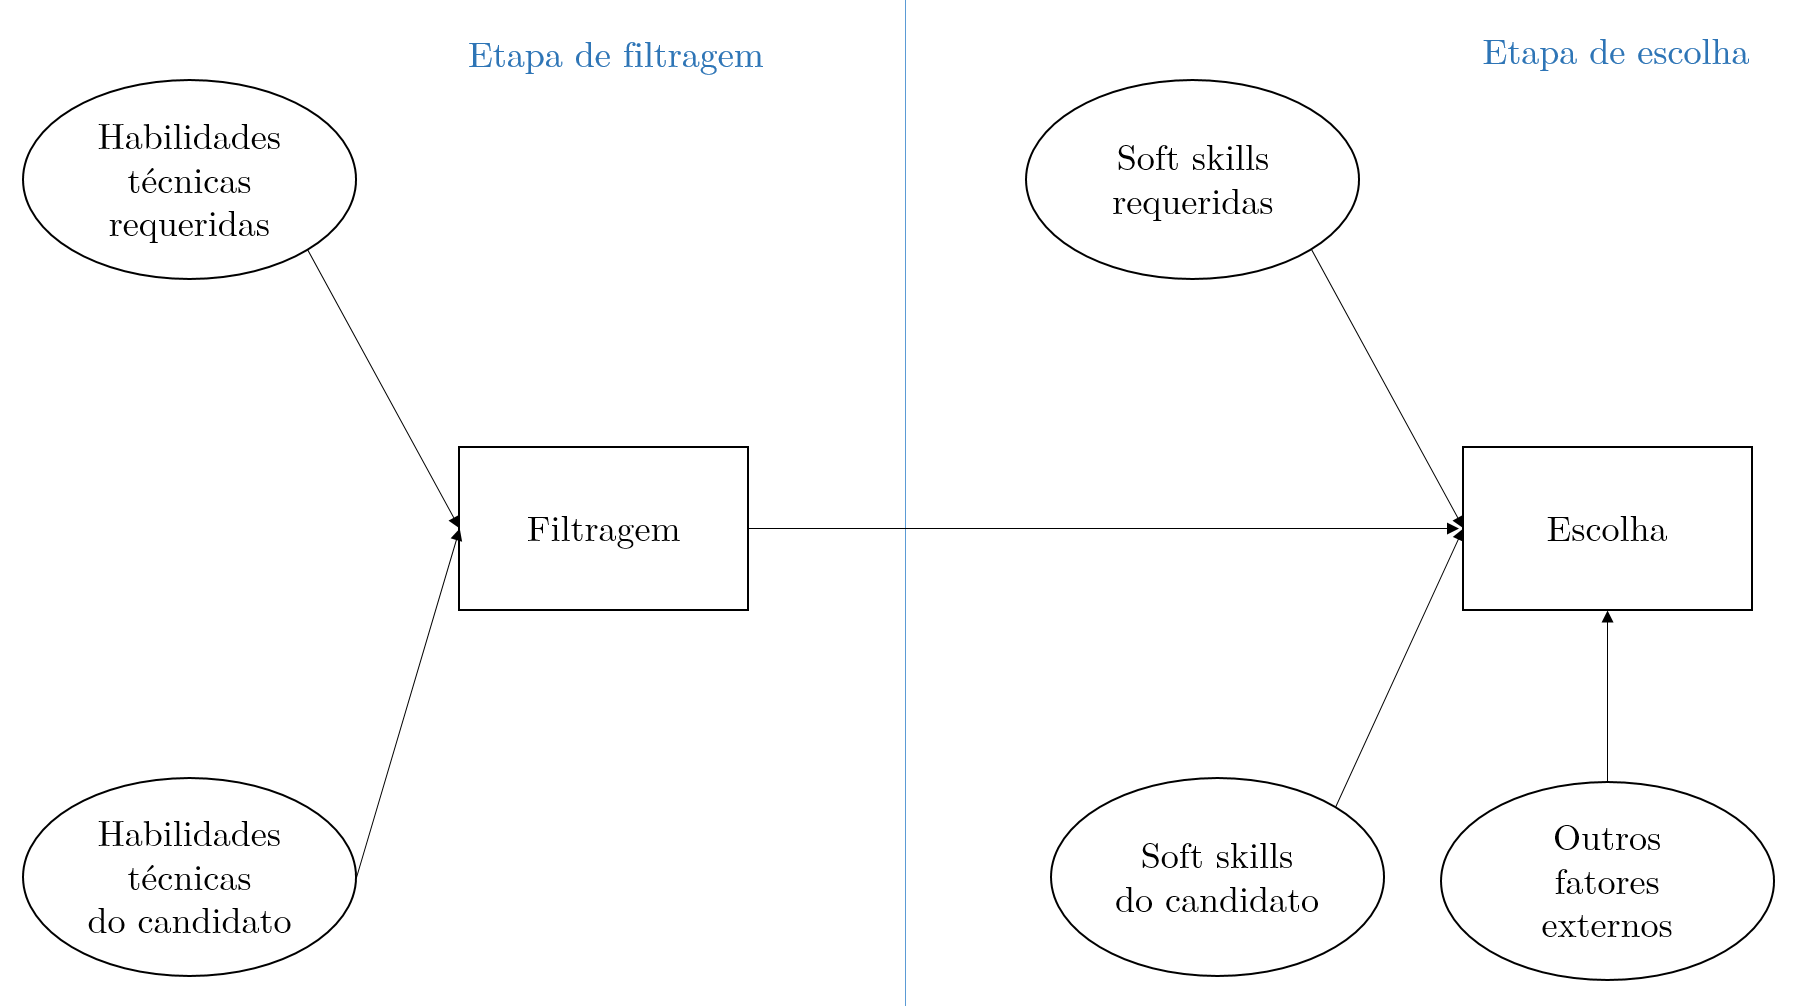
\includegraphics[width=.99\textwidth]{modelocontratacao.png}
\label{fig:modelocontratacao}
\fonte{\cite{litecky:04}} %\cite{litecky:04}} Precisa citar outra vez na imagem? 
\end{figure}

As habilidades técnicas são as características básicas procuradas em um profissional. Elas funcionam como um filtro. Normalmente, são utilizadas para eliminar um candidato que não está apto a um determinado cargo, de acordo com seu currículo. Portanto, as habilidades técnicas são importantes principalmente no processo de recrutamento dos candidatos.

Após o recrutamento, segue-se a fase de contratação. Nessa etapa, gerentes e profissionais de recursos humanos costumam dar mais atenção ao conjunto de habilidades não-técnicas que o candidato possui. Assim, as soft skills são diferenciais nessa etapa, fazendo com que o candidato se destaque entre os demais. Isso demonstra a importância da identificação das mesmas e a busca por desenvolver-se como um profissional com um conjunto mais amplo de habilidades, além das técnicas tradicionais.

Quando consideramos indivíduos ainda em formação educacional, que estão em busca de estágio, ou mesmo do primeiro emprego, conhecer e desenvolver soft skills é ainda mais crucial. Esses indivíduos são candidatos com pouca, ou nenhuma, experiência profissional. Portanto, as soft skills serão os valores mais importantes que os mesmos podem apresentar nessa etapa. Elas complementam sua formação teórica e podem fazer diferença para serem escolhidos e ocuparem os cargos desejados.

\section{Modelo dos Cinco Fatores}
\label{sec:ffm}

As teorias de personalidade têm objetivo de auxiliar no entendimento a respeitos dos interesses, comportamentos e características de cada indivíduo. Através dessa área da Psicologia, podemos buscar conceitos para entender melhor o que significa cada soft skill, tornando possível identificar como se comporta e quais características são expressas por um indivíduo que possui uma determinada habilidade. Em busca desse conhecimento, nesta seção explicamos o Modelo dos Cinco Fatores (Five Factor Model - FFM), que é uma teoria da Psicologia sobre personalidade.

O FFM é um modelo para descrever a personalidade através de uma estrutura de traços (traits), em termos de cinco dimensões básicas: Extroversão (Extraversion – E), Amabilidade (Agreeableness – A), Conscienciosidade (Conscientiousness - C), Neuroticismo (Neuroticism - N) e Abertura à experiência (Openness to Experience - O) \cite{mccrae:92}. Embora  existam  algumas  controvérsias com relação à denominação de cada fator, as traduções aqui colocadas estão de acordo com a nomenclatura utilizada na versão brasileira do manual Inventário de Personalidade NEO Revisado (NEO PI-R) \cite{flores:07}.

Os fatores definidos pelo FFM são comumente chamados de cinco grandes traços da personalidade, reconhecidos pelo termo ``Big Five’’. Cada um dos cinco fatores do modelo representa uma dimensão dentro da qual um indivíduo se encontra. Através de procedimentos de avaliação, como inventários de testes, cada fator é medido para definir os aspectos marcantes da personalidade \cite{costa:92b}.

O fator Extroversão mostra a tendência por buscar estímulo na companhia dos outros e no envolvimento com o mundo exterior. Pessoas que pontuam alto nesse fator são extrovertidas, ou seja, são cheias de energia, sociáveis e falantes. Quando uma baixa pontuação representa esse fator, o indivíduo é introvertido. Pessoas introvertidas precisam de mais tempo sozinho e buscam menos estímulos que as extrovertidas. Isso não significa que eles são antissociais, mas que são reservados e quietos.

Amabilidade é um fator que descreve o relacionamento interpessoal. Indivíduos que pontuam alto nesse fator valorizam conviver com os outros. Eles são amáveis, compreensivos e confiáveis. Já os que pontuam baixo, tendem a pensar sobre si mesmo, em vez dos outros, o que significa que eles valorizam o autointeresse. Normalmente, são críticos e briguentos.

O fator Conscienciosidade descreve pessoas autodisciplinadas. Indivíduos que pontual alto nesse fator apreciam planejamento e organização. Eles são persistentes e motivados para atingir seus objetivos. Também têm facilidade para prestar atenção a detalhes. Pelo contrário, os indivíduos com baixa Conscienciosidade são descuidados e desorganizados. Normalmente, se sentem confortável com comportamentos espontâneos, decisões em aberto e tarefas não cumpridas.

O fator Neuroticismo indica instabilidade emocional. É a tendência a experimentar emoções negativas, como ansiedade ou depressão. Aqueles que têm alta pontuação em Neuroticismo são emocionalmente vulneráveis ao estresse. Por outro lado, pontuações baixas definem pessoas calmas e emocionalmente estáveis.

Abertura à experiência define pessoas interessadas em aprender e explorar novas culturas. Indivíduos que tendem a apreciar imaginação e curiosidade. Normalmente, são criativos. Pessoas com baixa pontuação em Abertura à experiência tendem a ter interesses mais convencionais e tradicionais.

O Modelo dos Cinco Fatores é reconhecido por definir as dimensões fundamentais da personalidade e por sua aplicabilidade em diversos contextos e culturas. Desde os anos 1960, teoristas da área de Psicologia já buscavam propor um modelo que fosse capaz de definir a personalidade de forma geral e abrangente. No entanto, essa teoria demorou anos para ser estabelecida.

Pesquisas naquela época já reconheciam a ocorrência de cinco fatores \cite{tupes:61, norman:63}, mas apenas por volta dos anos 1980 começou a surgir um consenso a respeito da importância e do estabelecimento deles. Foi quando pesquisadores de diferentes tradições desenvolveram estudos a partir da análise da linguagem natural e utilização de questionários de personalidade, observando que os cinco fatores mostravam-se convergentes através de diferentes instrumentos e observadores \cite{mccrae:92}.

Os estudos com base na linguagem natural consistem em uma abordagem léxica de selecionar os termos de um dicionário % \{allport:00}
e agrupá-los em conjuntos de sinônimos, geralmente utilizando adjetivos para descrever cada dimensão. Esses adjetivos são maneiras de entender as características dos indivíduos através de termos que eles mesmos podem avaliar, servindo também para criar instrumentos de medição da personalidade \cite{goldberg:83, mccrae:85}. A Tabela \ref{tab:adjetivos} apresenta, por exemplo, uma lista de adjetivos, originalmente selecionados em inglês, para descrever cada dimensão do FFM, proposta por John (1989)\nocite{john:89} e referida por McCrae e John (1992)\nocite{mccrae:92}.

\begin{table*}[ht]
\footnotesize
\caption{\small Exemplos de adjetivos definindo os Cinco Fatores} 
\addtolength{\tabcolsep}{-3.5pt}
\renewcommand{\arraystretch}{1.4} 
\centering
	
		    \begin{tabular}{|c|l|l|}
    \hline %\toprule
    \textbf{Fator} & \textbf{Adjetivos (em inglês)} & \textbf{Adjetivos (tradução)} \\
    \hline %\midrule
    \multirow{6}[2]{*}{\textbf{Extroversão}} & Active & Ativo \\
          & Assertive & Assertivo \\
          & Energetic & Energético \\
          & Enthusiastic & Entusiasmado \\
          & Outgoing & Sociável \\
          & Talkative & Falante \\ \hline
    \multirow{6}[2]{*}{\textbf{Amabilidade}} & Appreciative & Apreciativo \\
          & Forgiving & Perdoador \\
          & Generous & Generoso \\
          & Kind  & Amável \\
          & Sympathetic & Compreensivo \\
          & Trusting & Confiante \\ \hline
		\multirow{6}[1]{*}{\textbf{Conscienciosidade}} & Efficient & Eficiente \\
          & Organized & Organizado \\
          & Planful & Planejado \\
          & Reliable & Confiável \\
          & Responsible & Responsável \\
          & Thorough & Minucioso \\ \hline
    \multirow{6}[0]{*}{\textbf{Neuroticismo}} & Anxious & Ansioso \\
          & Self-pitying & Autopiedoso \\
          & Tense & Tenso \\
          & Touchy & Sensível \\
          & Unstable & Instável \\
          & Worrying & Preocupado \\ \hline
    \multirow{6}[0]{*}{\textbf{Abertura à experiência}} & Artistic & Artístico \\
          & Curious & Curioso \\
          & Imaginative & Imaginativo \\
          & Insightful & Esclarecido \\
          & Original & Original \\
          & Wide interests & Interesses amplos \\
    \hline %\bottomrule
    \end{tabular}%
		\label{tab:adjetivos}
		\fonte{\cite{john:89, mccrae:92}} %\cite{john:89}, \cite{mccrae:92} Precisa citar novamente?
\end{table*}

%Um desses instrumentos foi proposto por Goldberg \cite{goldberg:83}, através de uma série de análises com base na língua inglesa, a partir da qual 40 pares de adjetivos que foram cuidadosamente selecionados e organizados em 5 grupos de 9 adjetivos cada.

Um reconhecido instrumento de medição da personalidade é o NEO PI-R (Revised NEO Personality Inventory), que trata-se de um questionário com base no Modelo dos Cinco Fatores \cite{costa:92a}. O questionário mede os fatores Neuroticismo, Extroversão, Abertura à experiência, Amabilidade e Conscienciosidade através de 240 declarações nas quais os indivíduos inquiridos utilizam uma escala de Likert de cinco pontos para avaliação (entre concordo fortemente e discordo fortemente).

A sigla NEO origina-se do nome do questionário em versões anteriores e significa ``Neuroticism-Extraversion-Openness'', referentes aos três primeiros fatores que originalmente eram avaliados na primeira versão (NEO Inventory - NEO-I, de 1978). Quando os outros dois fatores foram incluídos, resolveu-se manter a sigla para o nome do questionário que passou a chamar-se, em 1985, NEO Personality Inventory (NEO-PI) \cite{costa:85}. O NEO PI-R é uma versão revisada deste último e foi publicado em 1990. Há ainda uma versão reduzida do NEO PI-R, o NEO Five-Factor Inventory (NEO-FFI) \cite{costa:92b}, que utiliza 60 itens para avaliar as cinco dimensões da personalidade.

Os questionários NEO têm sido traduzidos e avaliados em muitas línguas e culturas diferentes. No Brasil, foi publicada uma versão traduzida do manual do NEO PI-R, intitulada Inventário de Personalidade NEO Revisado (NEO PI-R) \cite{flores:07}. As propriedades psicométricas do NEO PI-R têm se mostrado consistentes e o instrumento é considerado válido para generalização em diversas idades, culturas e métodos de medição \cite{mccrae:11}.

De acordo com o NEO PI-R, cada grande traço da personalidade é representado por seis facetas (facets), que podem ser definidas como um conjunto de traços mais específicos. As facetas possuem o papel de representar a amplitude e o alcance de cada fator \cite{mccrae:06}. No questionário NEO PI-R, para cada um dos cinco fatores, as seis facetas contam com oito declarações para responder a cada uma delas, totalizando 48 declarações para cada um dos cinco fatores, 240 declarações no total. Na Tabela \ref{tab:facetas} podemos ver as facetas respectivas a cada fator.

\begin{table*}[ht]
\footnotesize
\caption{\small Facetas distribuídas por fator} 
\addtolength{\tabcolsep}{-3pt}
\renewcommand{\arraystretch}{1.4} 
\centering

		\begin{tabular}{|c|c|c|c|c|c|}
		  \hline
			\textbf{Fator} & \textbf{Extroversão} & \textbf{Amabilidade} & \textbf{Conscienciosidade} & \textbf{Neuroticismo} & \textbf{Abertura}\\ \hline
			\textbf{Facetas}
										& \vtop{\hbox{\strut Acolhimento}
														\hbox{\strut Gregarismo}
														\hbox{\strut Assertividade}
														\hbox{\strut Atividade}
														\hbox{\strut Busca de sensações}
														\hbox{\strut Emoções positivas}}
										& \vtop{\hbox{\strut Confiança}
														\hbox{\strut Franqueza}
														\hbox{\strut Altruísmo}
														\hbox{\strut Aquiescência}
														\hbox{\strut Modéstia}
														\hbox{\strut Sensibilidade}}
										& \vtop{\hbox{\strut Competência}
														\hbox{\strut Ordem}
														\hbox{\strut Senso de dever}
														\hbox{\strut Direcionamento}
														\hbox{\strut Autodisciplina}
														\hbox{\strut Deliberação}}
										& \vtop{\hbox{\strut Ansiedade}
														\hbox{\strut Hostilidade}
														\hbox{\strut Depressão}
														\hbox{\strut Autoconsciência}
														\hbox{\strut Impulsividade}
														\hbox{\strut Vulnerabilidade}}
										& \vtop{\hbox{\strut Fantasia}
														\hbox{\strut Estética}
														\hbox{\strut Sentimentos}
														\hbox{\strut Ações}
														\hbox{\strut Ideias}
														\hbox{\strut Valores}}
		\\ \hline
		\end{tabular}
		\label{tab:facetas}
		\fonte{\cite{mccrae:06, flores:07}}
\end{table*}

Adicionalmente, existe uma breve medida de personalidade chamada TIPI (Ten-Item Personality Inventory), \cite{gosling:03}, que foi desenvolvida para avaliar os cinco fatores do FFM a partir de um pequeno questionário de apenas dez itens. Apesar de tratar-se de um instrumento mais simples, o TIPI atingiu níveis de convergência aceitáveis quando comparado com os grandes questionários. Portanto, é uma alternativa de medição da personalidade diante de situações onde os recursos e o tempo para avaliação são limitados.
